A metodologia adotada neste estudo consiste em um pipeline estruturado para a classificação automática dos graus ISUP em imagens histopatológicas de próstata, conforme ilustrado na Figura \ref{fig:methodology}. Inicialmente, o conjunto de dados PANDA é adquirido e submetido a etapas de pré-processamento, seguido pela divisão em treino e teste. Em seguida, aplica-se uma filtragem para redução de ruído, com o objetivo de remover imagens potencialmente inconclusivas que poderiam comprometer o processo de aprendizagem dos modelos. Após essa etapa, as lâminas completas são fragmentadas em patches, reduzindo a dimensionalidade espacial e tornando o treinamento computacionalmente mais eficiente. Na fase de modelagem, diferentes classificadores individuais são treinados empregando distintas estratégias de aprendizado. Por fim, utiliza-se uma abordagem de ensemble para combinar as predições desses modelos, resultando em uma solução mais robusta e estável.

\begin{figure}[H]
	\centering
	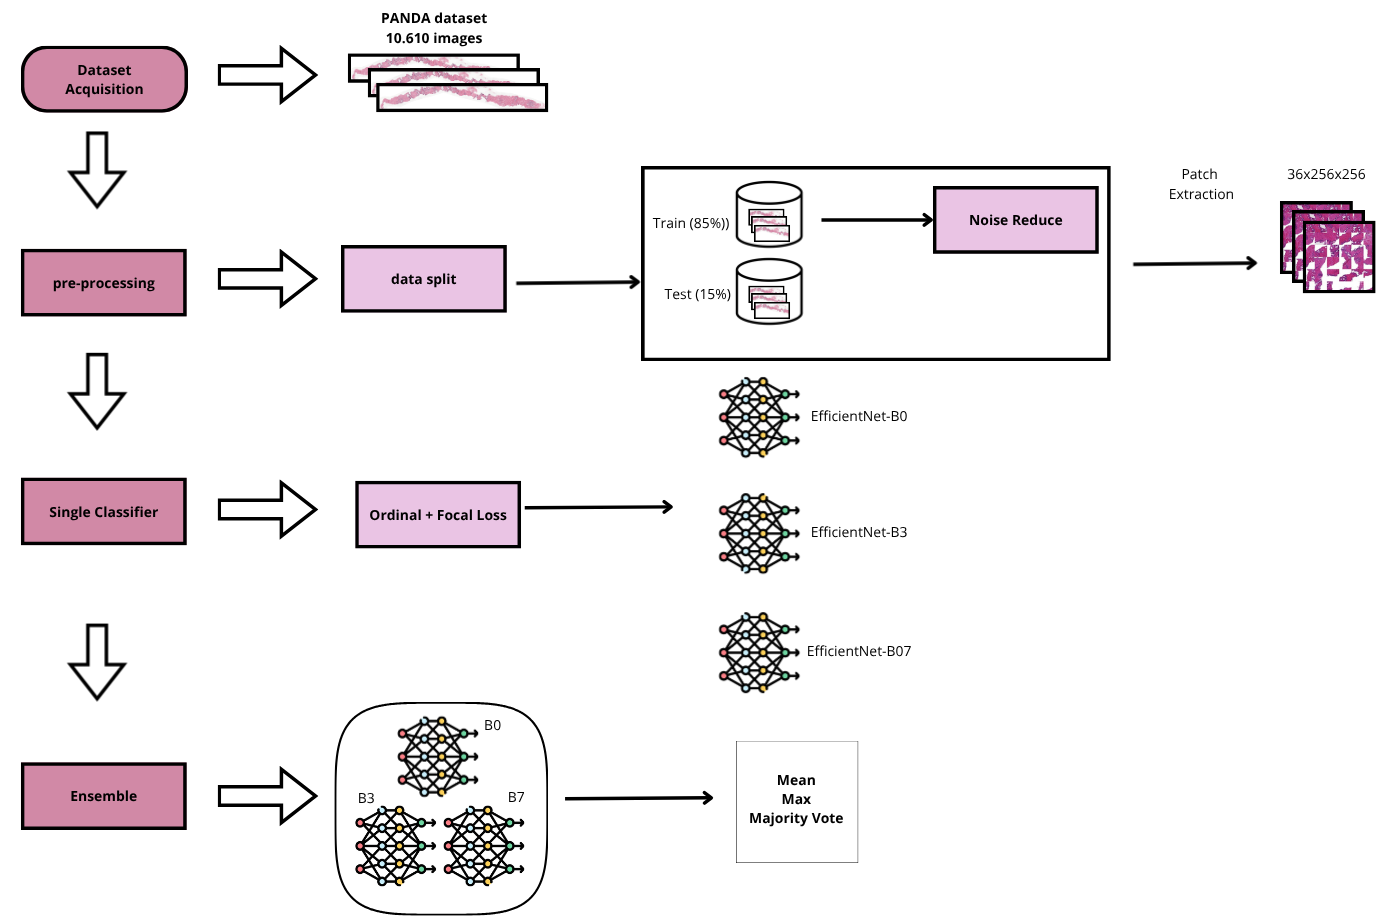
\includegraphics[width=1\linewidth]{images/methodology}
	\caption{}
	\label{fig:methodology}
\end{figure}


\subsection{Dataset Acquisition}

Utilizamos o conjunto de dados do Prostate cANcer graDe Assessment (PANDA)~\cite{ref-panda2020}, composto por 10.616 whole-slide images (WSIs) de biópsias de próstata digitalizadas em alta resolução (20×). Cada imagem foi anotada segundo o sistema de graduação ISUP (0–5), no qual o grau 0 indica ausência de malignidade, enquanto os graus 1 a 5 representam níveis crescentes de agressividade tumoral.

A Tabela~\ref{tab:dist_classes} apresenta a distribuição das classes do conjunto de dados. Observa-se um desbalanceamento significativo entre os rótulos, com predominância da classe 0 (aproximadamente 27\%). Em contraste, as classes associadas a graus clínicos mais avançados (ISUP 4 e 5) representam, cada uma, menos de 12\% do total.

As imagens do PANDA são provenientes de dois centros médicos distintos: Radboud University Medical Center e Karolinska Institutet. Segundo os autores~\cite{ref-panda2020}, as lâminas do Radboud foram anotadas por estudantes treinados, enquanto as do Karolinska foram rotuladas por patologistas experientes. Essa heterogeneidade introduz variabilidade interinstitucional nas anotações. Além disso, o conjunto público apresenta diferentes formas de ruído, incluindo anotações excessivamente inclusivas e marcas de caneta próximas a regiões tumorais, o que pode afetar a qualidade do treinamento dos modelos.

\begin{table*}[!ht]
	\centering
	\caption{Characteristics of the PANDA dataset used in this study.}
	\label{tab:panda_like}
	\begin{tabular}{l c c c}
		\hline
		& \textbf{Karolinska} & \textbf{Radboud} & \textbf{Total} \\
		\hline
		
		\textbf{ISUP Grade} & & & \\
		
		\quad 0 
		& 1,520 (27.9\%) & 1,372 (26.6\%) & 2,892 (27.24\%) \\
		
		\quad 1 
		& 1,404 (25.7\%) & 1,262 (24.4\%) & 2,666 (25.11\%) \\
		
		\quad 2 
		& 690 (12.6\%) & 653 (12.7\%) & 1,343 (12.65\%) \\
		
		\quad 3 
		& 635 (11.6\%) & 607 (11.8\%) & 1,242 (11.70\%) \\
		
		\quad 4 
		& 641 (11.7\%) & 608 (11.8\%) & 1,249 (11.77\%) \\
		
		\quad 5 
		& 566 (10.3\%) & 658 (12.7\%) & 1,224 (11.53\%) \\
		
		\hline
		
		Total & 5,456 (51.3\%) & 5,160 (48.7\%) & 10,616 \\
		
		\hline
		\label{tab:dist_classes}
		
	\end{tabular}
\end{table*}


\subsection{Preprocessing}

O processo de Pré-processamento e Filtragem de Dados Baseada em Dificuldade iniciou-se com a divisão estratificada do conjunto de dados original: 15\% das instâncias foram reservadas exclusivamente para o conjunto de Teste (avaliação final do modelo), enquanto os 85\% restantes foram destinados aos conjuntos de Treinamento e Validação.
No subconjunto maior (85\% do total), aplicou-se um Aumento de Dados (Data Augmentation) por meio de espelhamento vertical e horizontal em 50\% das amostras de forma aleatória, com o objetivo de aumentar a robustez do modelo.

Em seguida, foi realizada a análise de dificuldade das instâncias. Para isso, empregou-se uma ensemble composta por quatro modelos EfficientNet (B0, B1, B2 e B3), todos pré-treinados no ImageNet. Para cada imagem, calculou-se o escore médio de entropia produzido pelos quatro modelos. As Para definir a melhor estratégia de filtragem, foram conduzidos experimentos removendo 10\%, 5\% e 2\% das maiores entropias. 


A Tabela~\ref{tab:dataset-filter} apresenta a quantidade de dados antes e depois da filtragem. Do subconjunto inicial de Treinamento+Validação (85\% do dataset original), havia 9.025 instâncias, reduzidas para 8.844 após a remoção das amostras difíceis. Deste total final de 8.844 imagens, 20\% foram reservadas para Validação (1.769 imagens) e 80\% para Treinamento (7.075 imagens). O conjunto de Teste permaneceu inalterado com 1.590 instâncias.

\begin{table}[H]
	\centering
	\caption{Summary of entropy-based filtering.}
	\begin{tabular}{lcccc}
		\toprule
		\textbf{Step} & \textbf{Total} & \textbf{Training} & \textbf{Validation} & \textbf{Test} \\
		\midrule
		Before filtering & 9025 & 7220 & 1805 & 1590 \\
		After filtering & 8844 & 7075 & 1769 & 1590 \\
		\bottomrule
	\end{tabular}
	\label{tab:dataset-filter}
\end{table}



\subsubsection{Patch extraction}
Considerando o tamanho das WSIs e a presença de áreas não informativas, foi aplicado um pré-processamento para otimizar o uso computacional e preservar regiões relevantes para o diagnóstico. Inicialmente, foram extraídos patches fixos de 256 × 256 pixels, selecionados com base em critérios empíricos de intensidade média e saturação nos canais RGB, a fim de eliminar regiões de fundo, artefatos e áreas sem coloração diagnóstica. A Figura~\ref{fig:origin-tiles} ilustra a imagem histopatológica original utilizada como base para a extração dos patches e a imagem composta resultante após a extração e o rearranjo dos patches, permitindo uma compreensão visual do processo.

\begin{figure}[!htb]
	\centering
	\subfloat[\centering Original]{{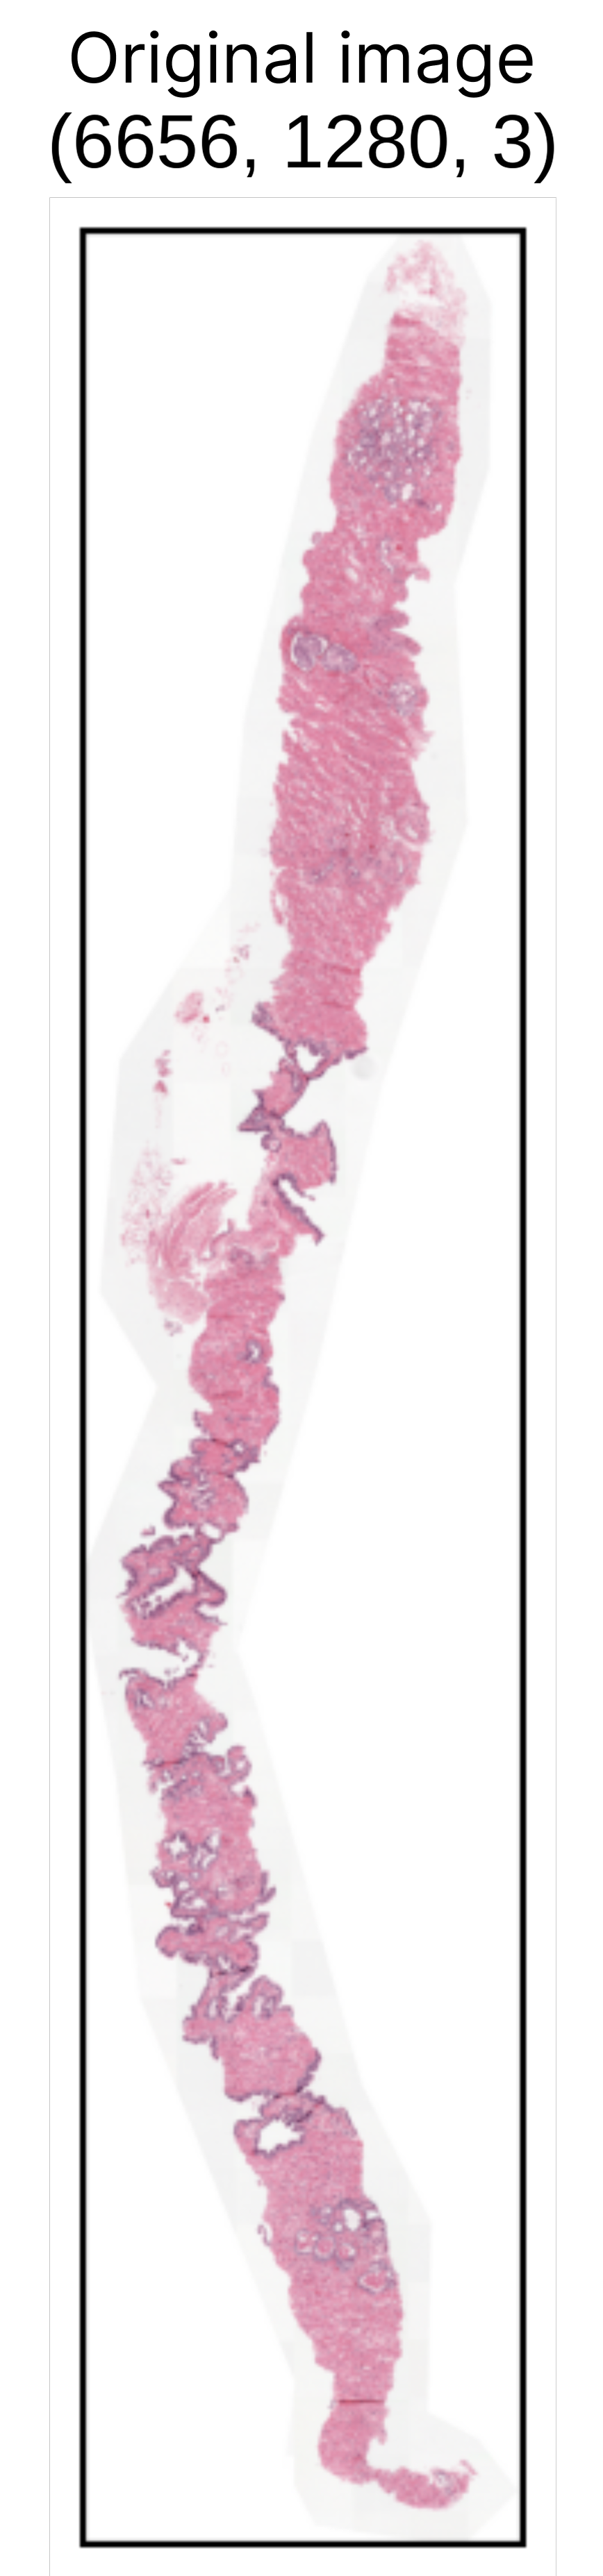
\includegraphics[width=0.1\textwidth, height=0.24\textheight]{images/original.png} }}%
	\qquad
	\subfloat[\centering Patched image]{{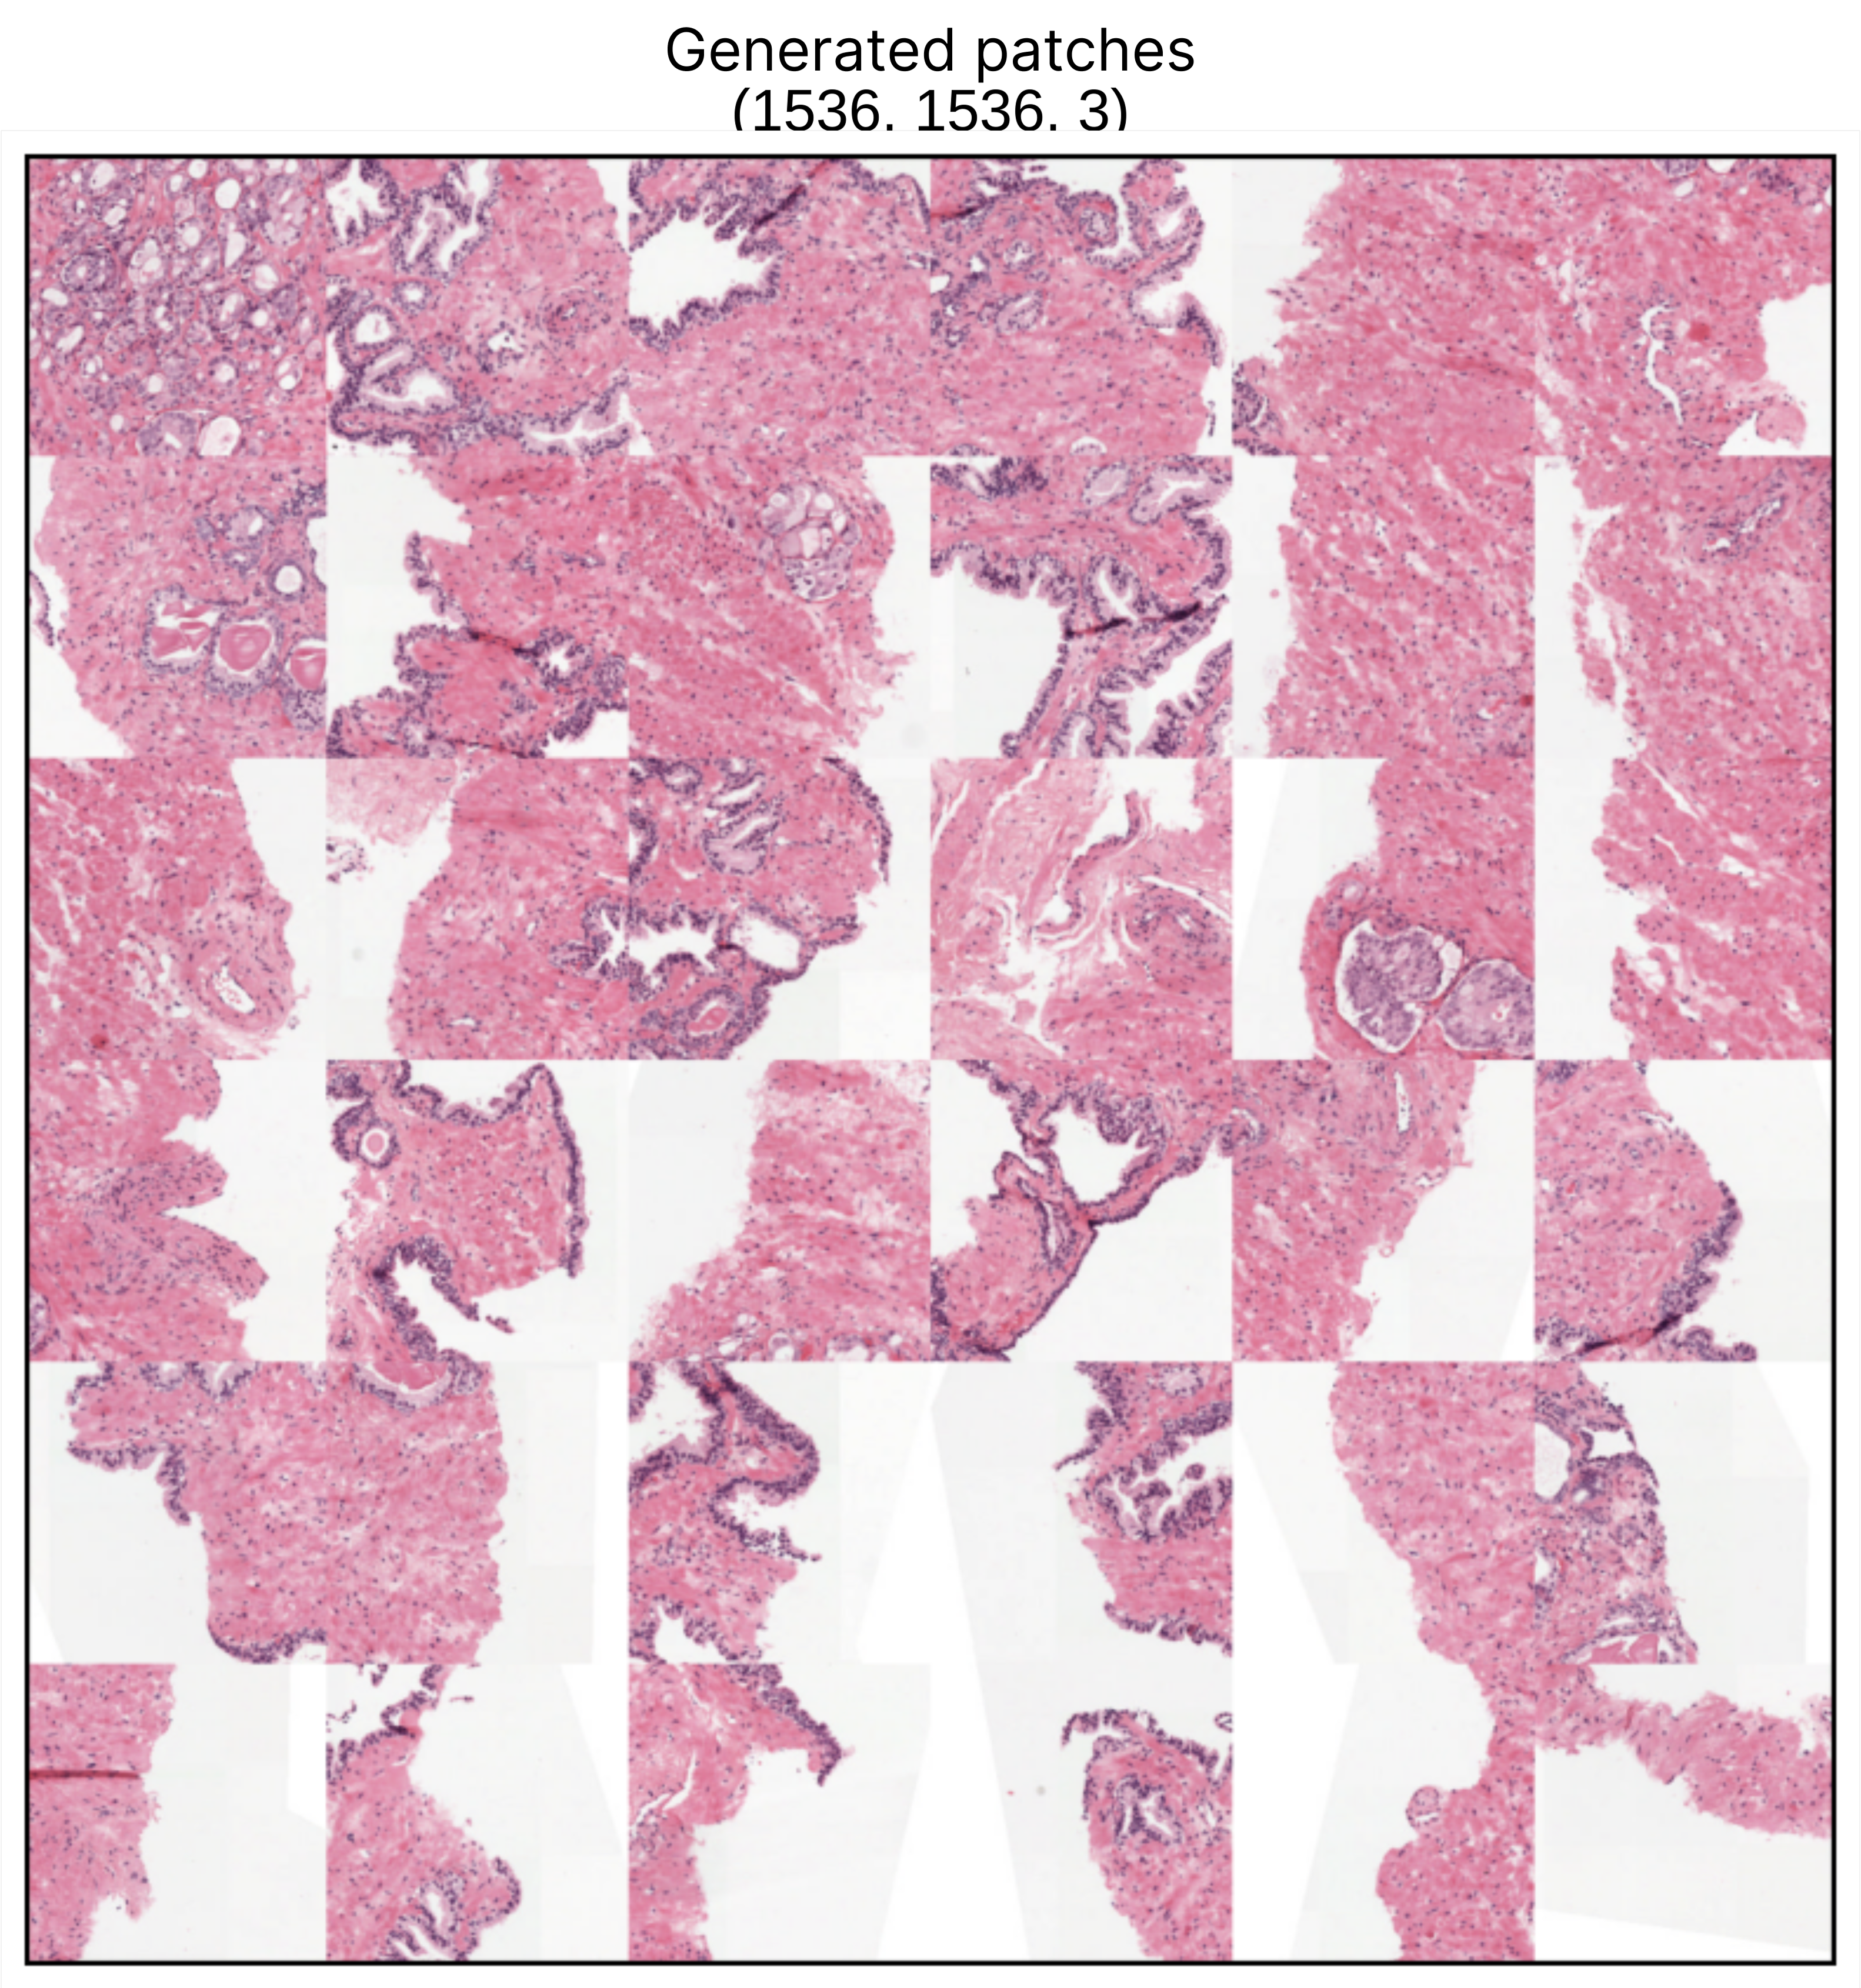
\includegraphics[width=0.33\textwidth,height=0.24\textheight]{images/tiles.png} }}%
	\caption{Original histopathological image (a) and composite image after patch extraction and rearrangement (b).}
	\label{fig:origin-tiles}
\end{figure}

Para cada lâmina, foram extraídos 36 patches, número definido por meio de experimentos preliminares que avaliaram o impacto da quantidade de regiões na representatividade morfológica e na viabilidade computacional. Para estabelecer essa escolha, três configurações foram comparadas: 25, 36 e 49 patches por lâmina, conforme ilustrado na Figura~\ref{fig:tiles-original}.

\begin{figure}[!htb]
	\centering
	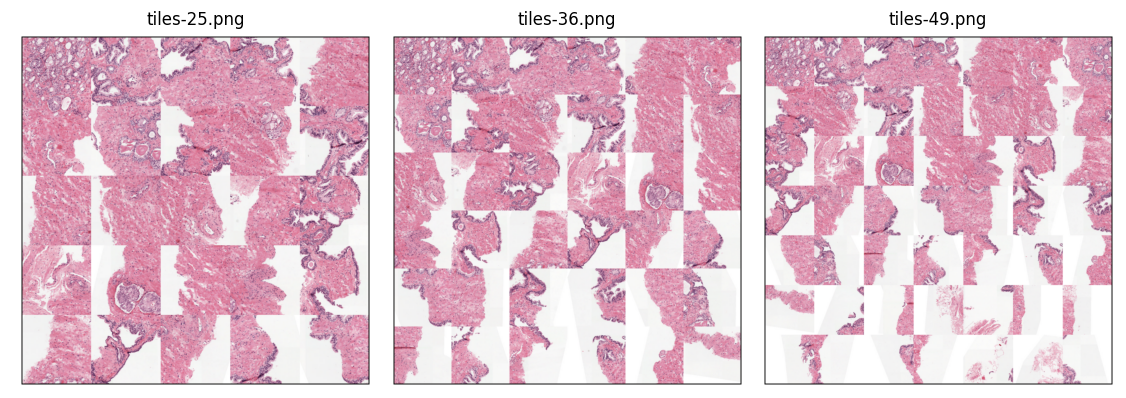
\includegraphics[width=0.5\textwidth]{images/tiles-original.png}
	%
	\caption{Representação da extração de patches com diferentes quantidades. A imagem contém três exemplos: (a) com 25 patches, (b) com 36 patches e (c) com 49 patches, exibidos da esquerda para a direita.}
	\label{fig:tiles-original}%
\end{figure}

A extração com 25 patches produziu uma composição compacta, consequentemente gerando menos dados a serem analisados, o que pode reduzir a demanda por recursos computacionais durante o treinamento e a validação do modelo. Entretanto, essa configuração limita a cobertura da lâmina, resultando em perda significativa de padrões morfológicos relevantes para a classificação. Por outro lado, a extração com 49 patches ampliou a área analisada, mas aumentou os custos computacionais e de armazenamento, além de incluir muitas regiões vazias ou redundantes que podem afetar a eficiência do processamento. Adicionalmente, a inclusão de áreas periféricas com baixo conteúdo discriminativo pode comprometer a qualidade da representação ao diluir ou saturar características importantes.

Assim, a configuração intermediária com 36 patches equilibra adequadamente a cobertura da diversidade morfológica e a eficiência computacional, abrangendo a maior parte das informações relevantes sem sobrecarregar a imagem com regiões irrelevantes. Por essa razão, essa configuração foi adotada como padrão neste trabalho. Após a extração, os patches foram reorganizados e concatenados em uma única imagem composta. Diferentemente de abordagens que preservam a distribuição espacial original, neste estudo os patches foram ordenados com base na quantidade de informação morfológica contida em cada um, estimada a partir de medidas de intensidade e saturação nos canais RGB.

\subsection{Single Classifier}
\subsection{Ensemble}
